% auteur: Dorian VOLPE

\begin{frame}
  \frametitle{Hashed Timelock Contract (HTLC)}
\begin{itemize}
  \item Ne nécessite pas de de tiers de confiance
  \item Réduit le risque de perte si l'on suit le protocole
  \item Verrouille les fonds dans un portefeuille qui peut être révoqué en cas de problème
\end{itemize}
\end{frame}

\begin{frame}
  \frametitle{HTLC fonctionnement - 1/2}
  \begin{itemize}
    \item Alice génère un hachage à partir de sa clé privée et l’envoie à Bob
    \item Elle génère également une pré-image du hachage en créant une transaction
    \item Bob génère également un hachage à partir de sa clé et l’envoie à Alice
    \item Une fois que Bob reçoit la transaction d’Alice, il signe la transaction en utilisant la clé originale qui est déjà disponible avec lui dans la pré-image
    \item Si Bob ne signe pas la transaction dans le temps imparti, la transaction est annulée et les fonds sont retournés à Alice
  \end{itemize}
\end{frame}

\begin{frame}
  \frametitle{HTLC fonctionnement - 2/2}
  \begin{figure}
    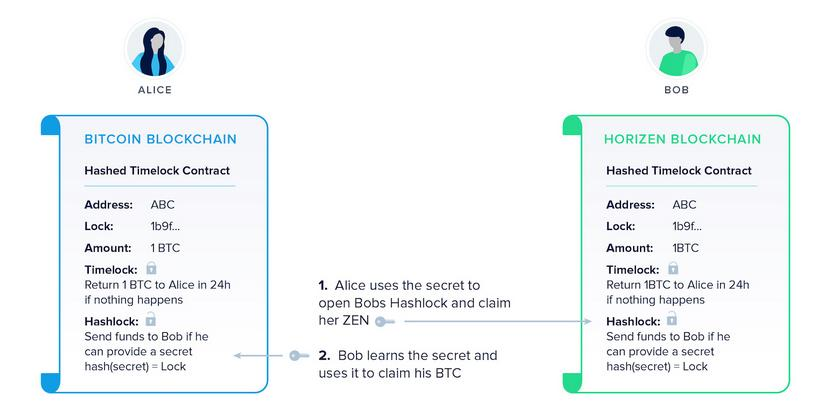
\includegraphics[scale = 0.4]{decentralisation/aliceBob.jpg}
    \caption[short]{Zoom sur les HTLC}
  \end{figure}
  
\end{frame}

\begin{frame}
  \frametitle{Atomic Swaps}
  Un swap atomique permet un échange de cryptomonnaies de blockchains séparées.
  \newline 
  \begin{itemize}
    \item Effectué entre deux entités sans l’intervention d’un tiers.
    \item L’idée est de supprimer les intermédiaires centralisés comme les échanges réglementés et de donner aux propriétaires de jetons un contrôle total.
    \item Utilise les HTLC. \newline
  \end{itemize}
    Deux propriétaires de cryptoactifs acceptent d’échanger leurs jetons pour une quantité donnée
  $\Rightarrow$ notion de connecteur publique.
\end{frame}

\begin{frame}
  \frametitle{Atomic Swaps - Exemple}
  \begin{figure}
    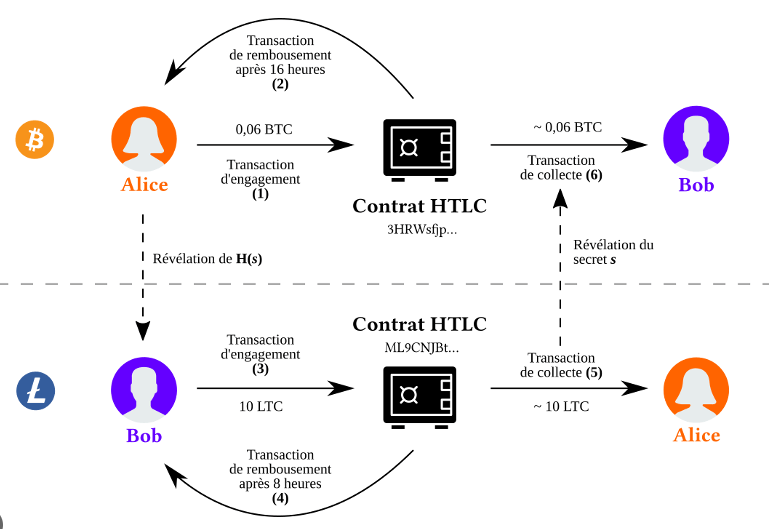
\includegraphics[scale = 0.35]{decentralisation/atomicswap.png}
  \caption{Processus d'échange atomique avec HTLC}
  \end{figure}
  
\end{frame}

\begin{frame}
  \frametitle{Atomic Swaps - Avantages}
  \subtitle{Avantages}
  \begin{itemize}
    \item Réduction des couts de transaction.
    \item Échange pair à pair sans tiers de confiance $\Rightarrow$ réellement décentralisé.
    \item Protection des échanges:
    \begin{itemize}
      \item Si un tiers suit le protocole il est assuré de ne pas perdre d'argent.
    \item Si jamais il ne suit pas le protocole il perd sa mise.
    \end{itemize} 
  \end{itemize}
\end{frame}

\begin{frame}
  \frametitle{Le réseau Lightning (Lightning Network)}
  \begin{itemize}
    \item Couche secondaire de la blockchain Bitcoin \newline
    \item Permet de faire des transactions en dehors de la blockchain principale $\Rightarrow$ off-chain
  \end{itemize}
\end{frame}

\begin{frame}
  \frametitle{Le réseau Lightning (Lightning Network) - Fonctionnement 1/2}
  Grâce à une transaction Bitcoin, deux noeuds du réseau peuvent construire un canal bidirectionnel sur lequel ils déposent une certaine quantité de bitcoins.
  \newline
  Les deux parties peuvent effectuer des transactions entre elles sans les diffuser sur le réseau Bitcoin.
  
\end{frame}

\begin{frame}
  \frametitle{Le réseau Lightning (Lightning Network) - Fonctionnement 2/2}
  \centering
  \begin{figure}
    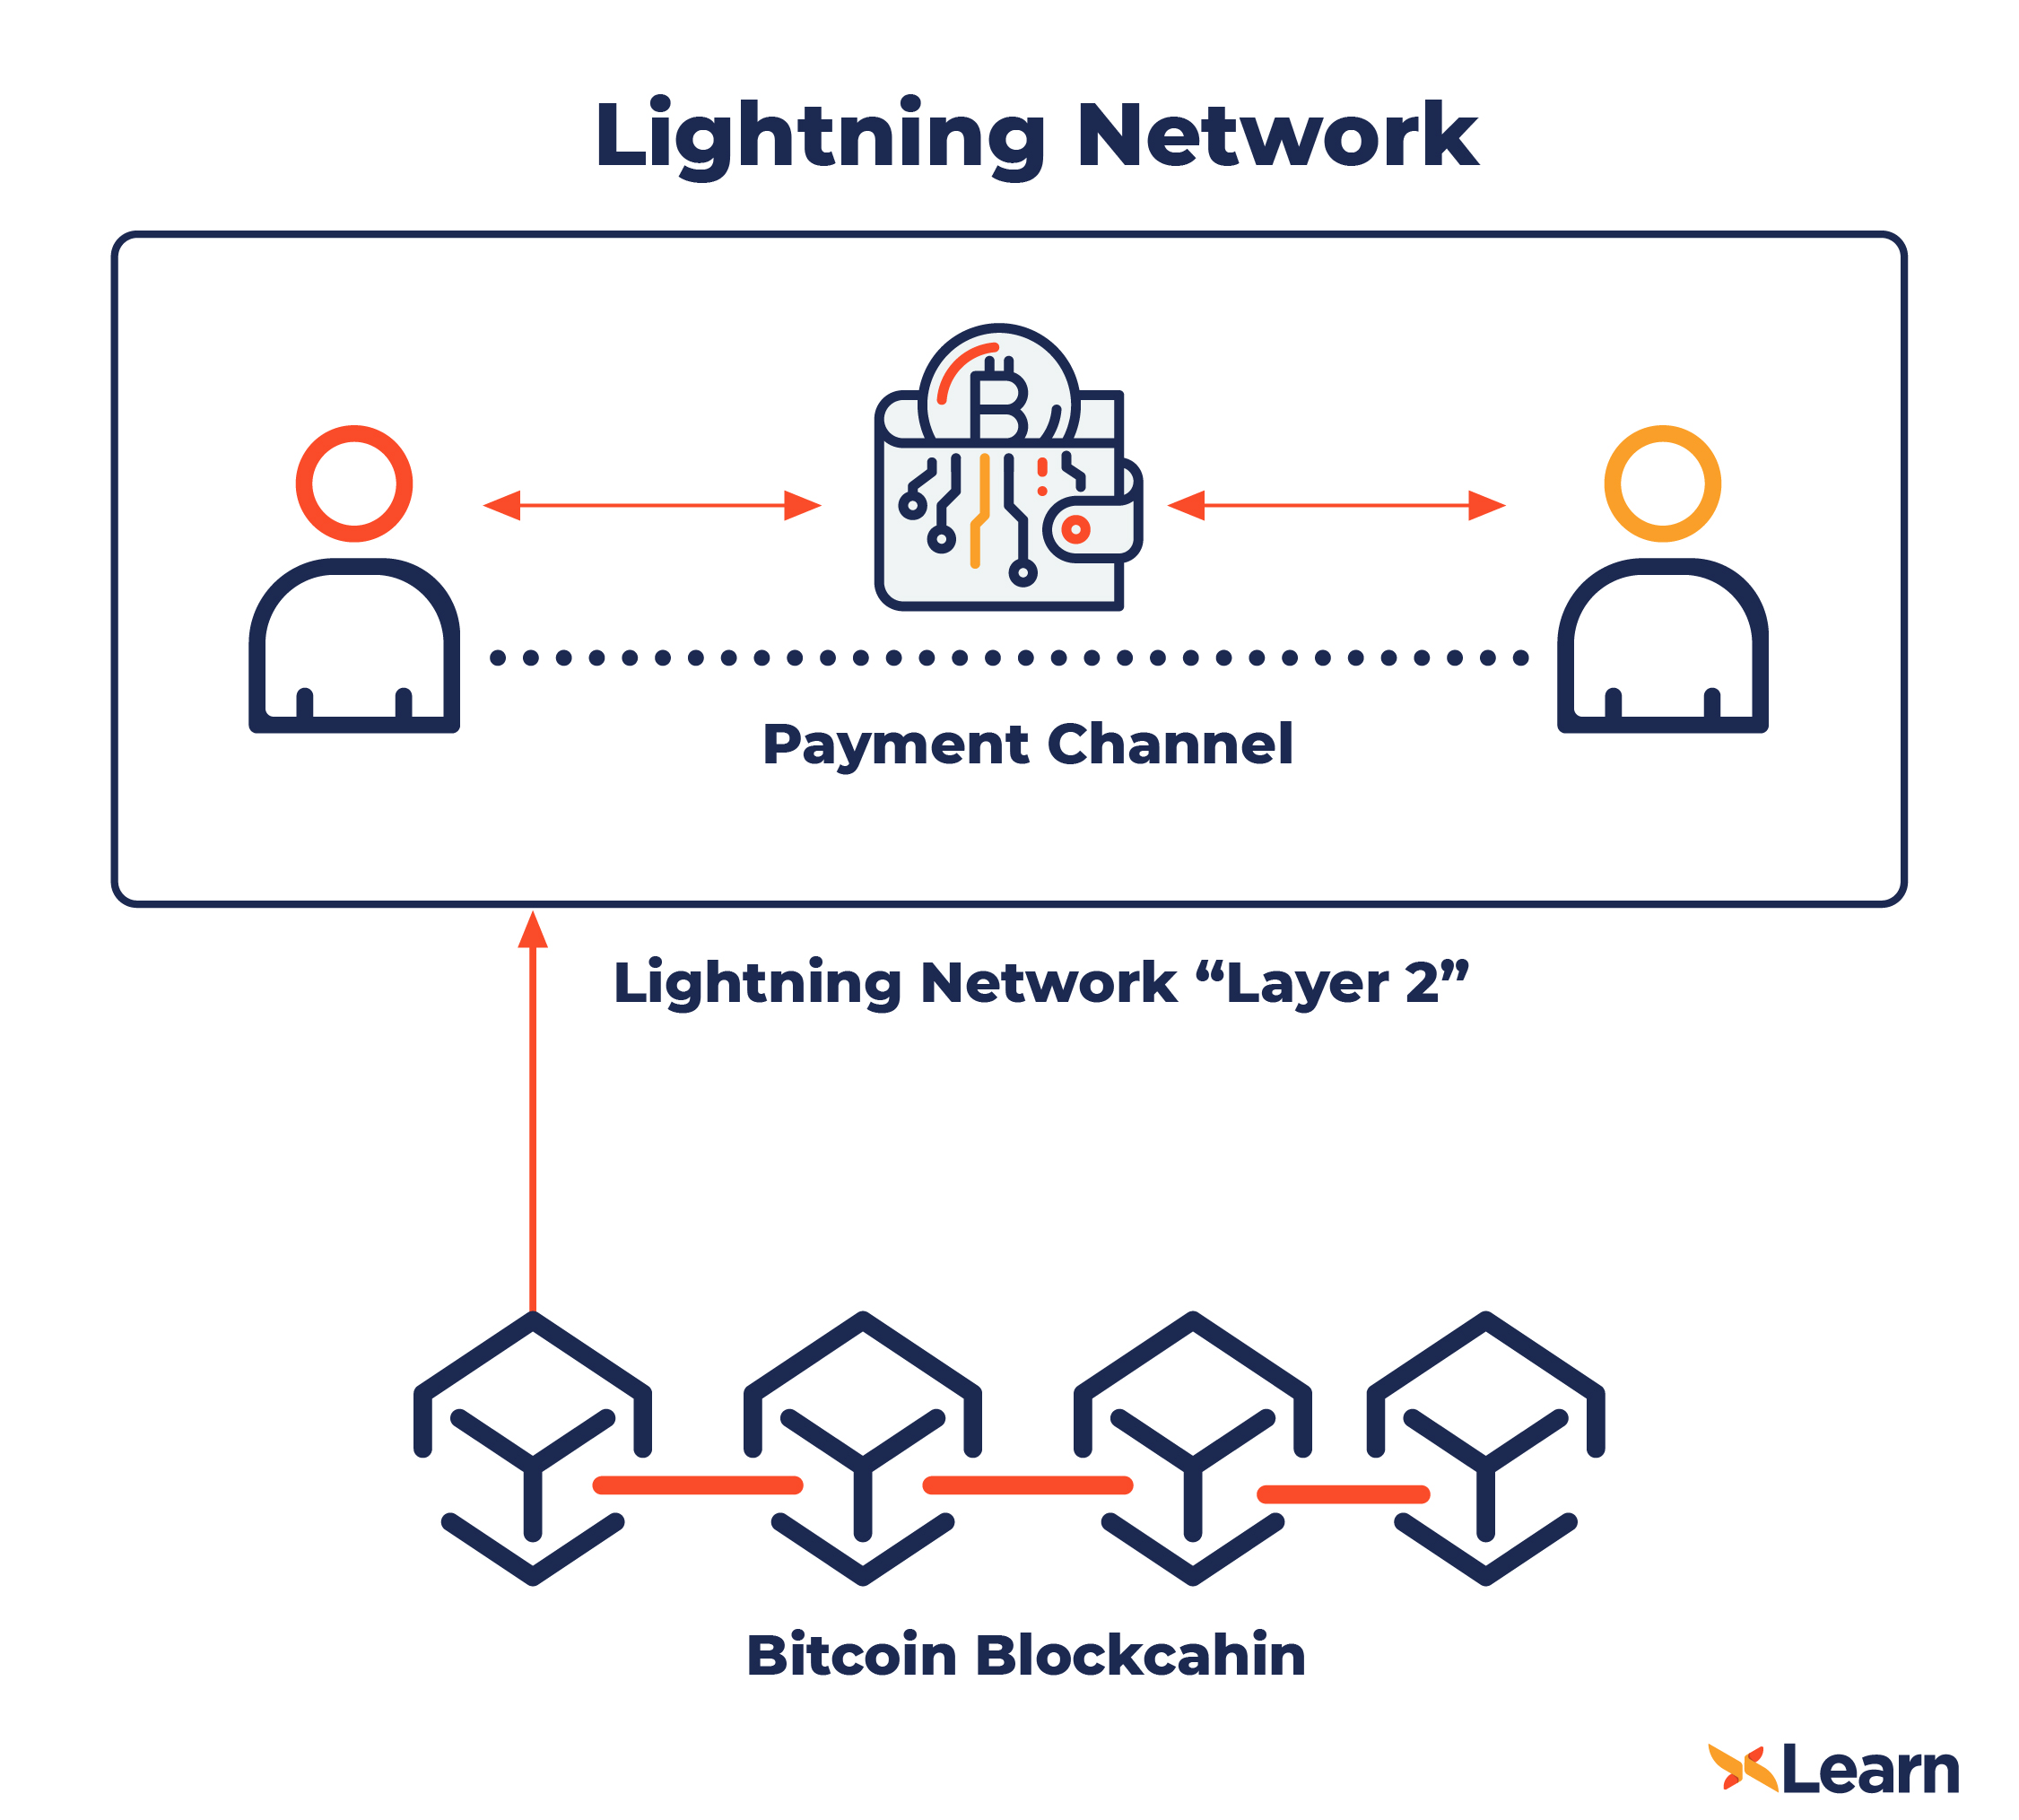
\includegraphics[scale = 0.24]{decentralisation/lightning.jpg}
  \end{figure}
  
\end{frame}

\begin{frame}
  \frametitle{Le réseau Lightning (Lightning Network) - Avantages}
  \begin{itemize}
    \item Aucune limite sur le nombre de transactions par seconde sur le réseau.
    \newline
    \item Des transactions instantanées. Plus d’attente de confirmation par les mineurs.
    \newline
    \item Des frais de transaction extrêmement faibles ouvrant la voie aux micro-transactions.
  \end{itemize}
\end{frame}

\begin{frame}
  \frametitle{Implémentation du MIT}
Implémentaion des swaps atomiques sur le réseau Lightning par le MIT. Les objectifs sont :
\newline
\begin{itemize}
  \item Permettre d'utiliser le réseau Lightning sur des blockchains différentes.
  \item Permettre des échanges sur des blockchains non monétaires \footnote{blockchains d'informations, de données,etc...}.
  \item Proposer une interface pour des échanges cross-chain.
\end{itemize}  

\end{frame}

\begin{frame}
  \frametitle{Implémentation du MIT - Nouvelles commandes 1/3}
  \begin{block}{Price}
    Commande de canal simple qui permet aux utilisateurs de rechercher la valeur marchande actuelle en USD de toute crypto-monnaie. 
  \end{block}
  \begin{block}{Compare}
    Récupère  la valeur marchande actuelle de chaque devise souhaitée et effectue une
   simple opération arithmétique pour retourner la valeur comparée entre elles.
  \end{block}
  
\end{frame}

\begin{frame}
  \frametitle{Implémentation du MIT - Nouvelles commandes 2/3}
  \begin{block}{Exchange}
Demande aux acteurs de la transaction d'alimenter un canal avec les montants souhaités. AVant de procéder à l'échange lui même.  
\end{block}
  \centering
  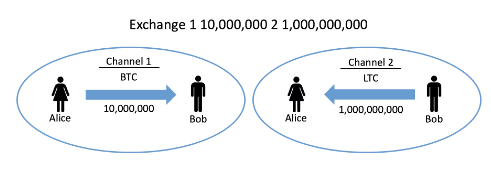
\includegraphics[scale = 0.6]{decentralisation/exchange.png}

\end{frame}

\begin{frame}
  \frametitle{Implémentation du MIT - Nouvelles commandes 3/3}
  \begin{block}{Respond}
    À ce stade de l'échange, Bob a une minute pour décider d'une action vis-à-vis de la demande d’échange d’Alice. Il peut faire l’une des trois choses suivantes : répondre oui et accepter l’échange, répondre non et le refuser, ou laisser la demande en "time out".  
  \end{block}
  $\Rightarrow$ On retrouve ici le principe des HTLC
\end{frame}

\begin{frame}
  \frametitle{Implémentation du MIT - Limitations}
  
  Il y a plusieurs limitation a cette Implémentaion:
  \newline
  \begin{itemize}
    \item Il n'y a pas de support de channel hopping \footnote{Transitivité des échanges entres plusieurs participants.} malgrès l'utilisation du réseau Lightning.
    \begin{itemize}
      \item Cela implique des problème de mise a l'échelle.
    \end{itemize}
    \item Il n'y a pas de vérification sur les valeurs inscrites sur les chaines non monétaires.
  \end{itemize}
\end{frame}
